\chapter{Detectores ópticos y calibración}
Los telescopios son instrumentos esenciales para observar objetos distantes en el cielo. Sin embargo, por sí solos no son suficientes para llevar a cabo un análisis detallado de los datos astronómicos. Para ello, es necesario contar con un dispositivo capaz de registrar todo lo que se observa a través del telescopio, permitiendo almacenar la información para su consulta y análisis posterior tantas veces como sea necesario, facilitando así la realización de un estudio riguroso. Estos dispositivos, denominados "detectores", son fundamentales en la astronomía moderna. En el rango óptico, los detectores más utilizados son los dispositivos de carga acoplada (CCD, por sus siglas en inglés). En esta clase, analizaremos algunas de sus características, así como las fuentes de ruido que generan y los métodos para reducirlas.


\section{Detectores ópticos}

\subsection{Semiconductores}
El funcionamiento de los detectores ópticos está basado en algunas de las propiedades de los materiales semiconductores. Por lo tanto, vale la pena hablar un poco sobre ellos. De manera simple, un semiconductor es un material que tiene propiedades intermedias entre un buen conductor de electricidad (como el cobre) y un buen aislante eléctrico (como el plástico). 

Los materiales que están compuestos por un mismo elemento pueden ser modelados a partir de redes o arreglos cristalinos, donde la separación entre cada átomo es fija y única para cada elemento. Así como los átomos individuales tienen niveles de energía permitidos para los electrones, los materiales (compuestos por muchos átomos del mismo elemento) tienen <<bandas>> de energía para los electrones. 

En la figura \ref{fig:valence-bands} se muestra un esquema de las bandas de energía para diferentes tipos de materiales. Los electrones más internos se mantienen ligados al núcleo (no hay una banda). En cambio los electrones más externos pueden interactuar para unir a los átomos (y formar estructuras), y se encuentran en las bandas de energía. La primer banda es llamada la banda de valencia, y la siguiente es conocida como la banda de conducción. 

\begin{figure}[htb]
  \centering
				\includegraphics[width=\textwidth]{figures/energy_bands.png}
				\caption{Bandas de valencia y conducción en los materiales}
				\label{fig:valence-bands} 
\end{figure}

En un aislante, la banda de valencia está completamente llena, mientras que la banda de conducción está totalmente vacía y la brecha entre ambas bandas es muy grande (panel izquierdo); los electrones tienen muy poca probabilidad de saltar de la banda de valencia a la de conducción. En un semiconductor, la banda de valencia está llena, mientras que la banda de conducción está vacía, pero ahora la brecha entre ambas bandas es pequeña y los electrones sí pueden saltar de una banda a otra (panel central). Finalmente, en un conductor, la banda de valencia también está completamente llena, mientras que la banda de conducción también contiene electrones, haciendo fácil el movimiento de cargas eléctricas (panel derecho). 

Cuando un electrón salta de la banda de valencia a la banda de conducción, éste deja una vacante, a la que se le suele llamar \emph{hueco}. Un electrón de un átomo cercano puede moverse hacia ese hueco, dejando así un nuevo hueco, que puede ser ocupado por otro electrón de otro átomo, y así sucesivamente. En este sentido, el hueco puede desplazarse por el material y se comporta como una corriente de carga positiva. Una manera de generar huecos es gracias al efecto fotoeléctrico, del que hablaremos a continuación. 

\subsubsection{Efecto fotoeléctrico}
El efecto fotoeléctrico es un fenómeno en el que los electrones son expulsados ​​de la superficie de un material conductor o semiconductor cuando la luz incide sobre él. Este efecto ocurre porque los electrones en la superficie del material pueden absorber la energía de la luz y usarla para superar la fuerza de atracción que los mantiene ligados al material. \citet{einstein1905heuristic} fue el primero en lograr explicar este fenómeno asumiendo que la luz está formada por partículas (los fotones) y gracias a eso obtuvo el Premio Nobel de Física en 1921. Además, sus resultados junto con la descripción de Planck del cuerpo negro fundaron las bases para la física cuántica. 

Para que ocurra el efecto fotoeléctrico, la luz debe ser lo suficientemente energética para hacer que los electrones escapen de la superficie. La cantidad mínima necesaria de energía que deben absorber los electrones para escapar depende de cada material y es conocida como la función de trabajo de la superficie, se representa con el símbolo $ \phi $. En otras palabras, el efecto fotoeléctrico ocurre únicamente si los fotones de la luz incidente tienen una energía $ h\nu \geq \phi $.

En la Figura \ref{fig:photo-effect} se muestra un esquema del efecto fotoeléctrico. La luz del panel izquierdo del esquema no tiene la energía suficiente para desprender a los electrones de la superficie. En cambio, la luz en el panel derecho del esquema sí y por lo tanto los electrones son expulsados de la superficie del material.  

\begin{figure}[htb]
  \centering
				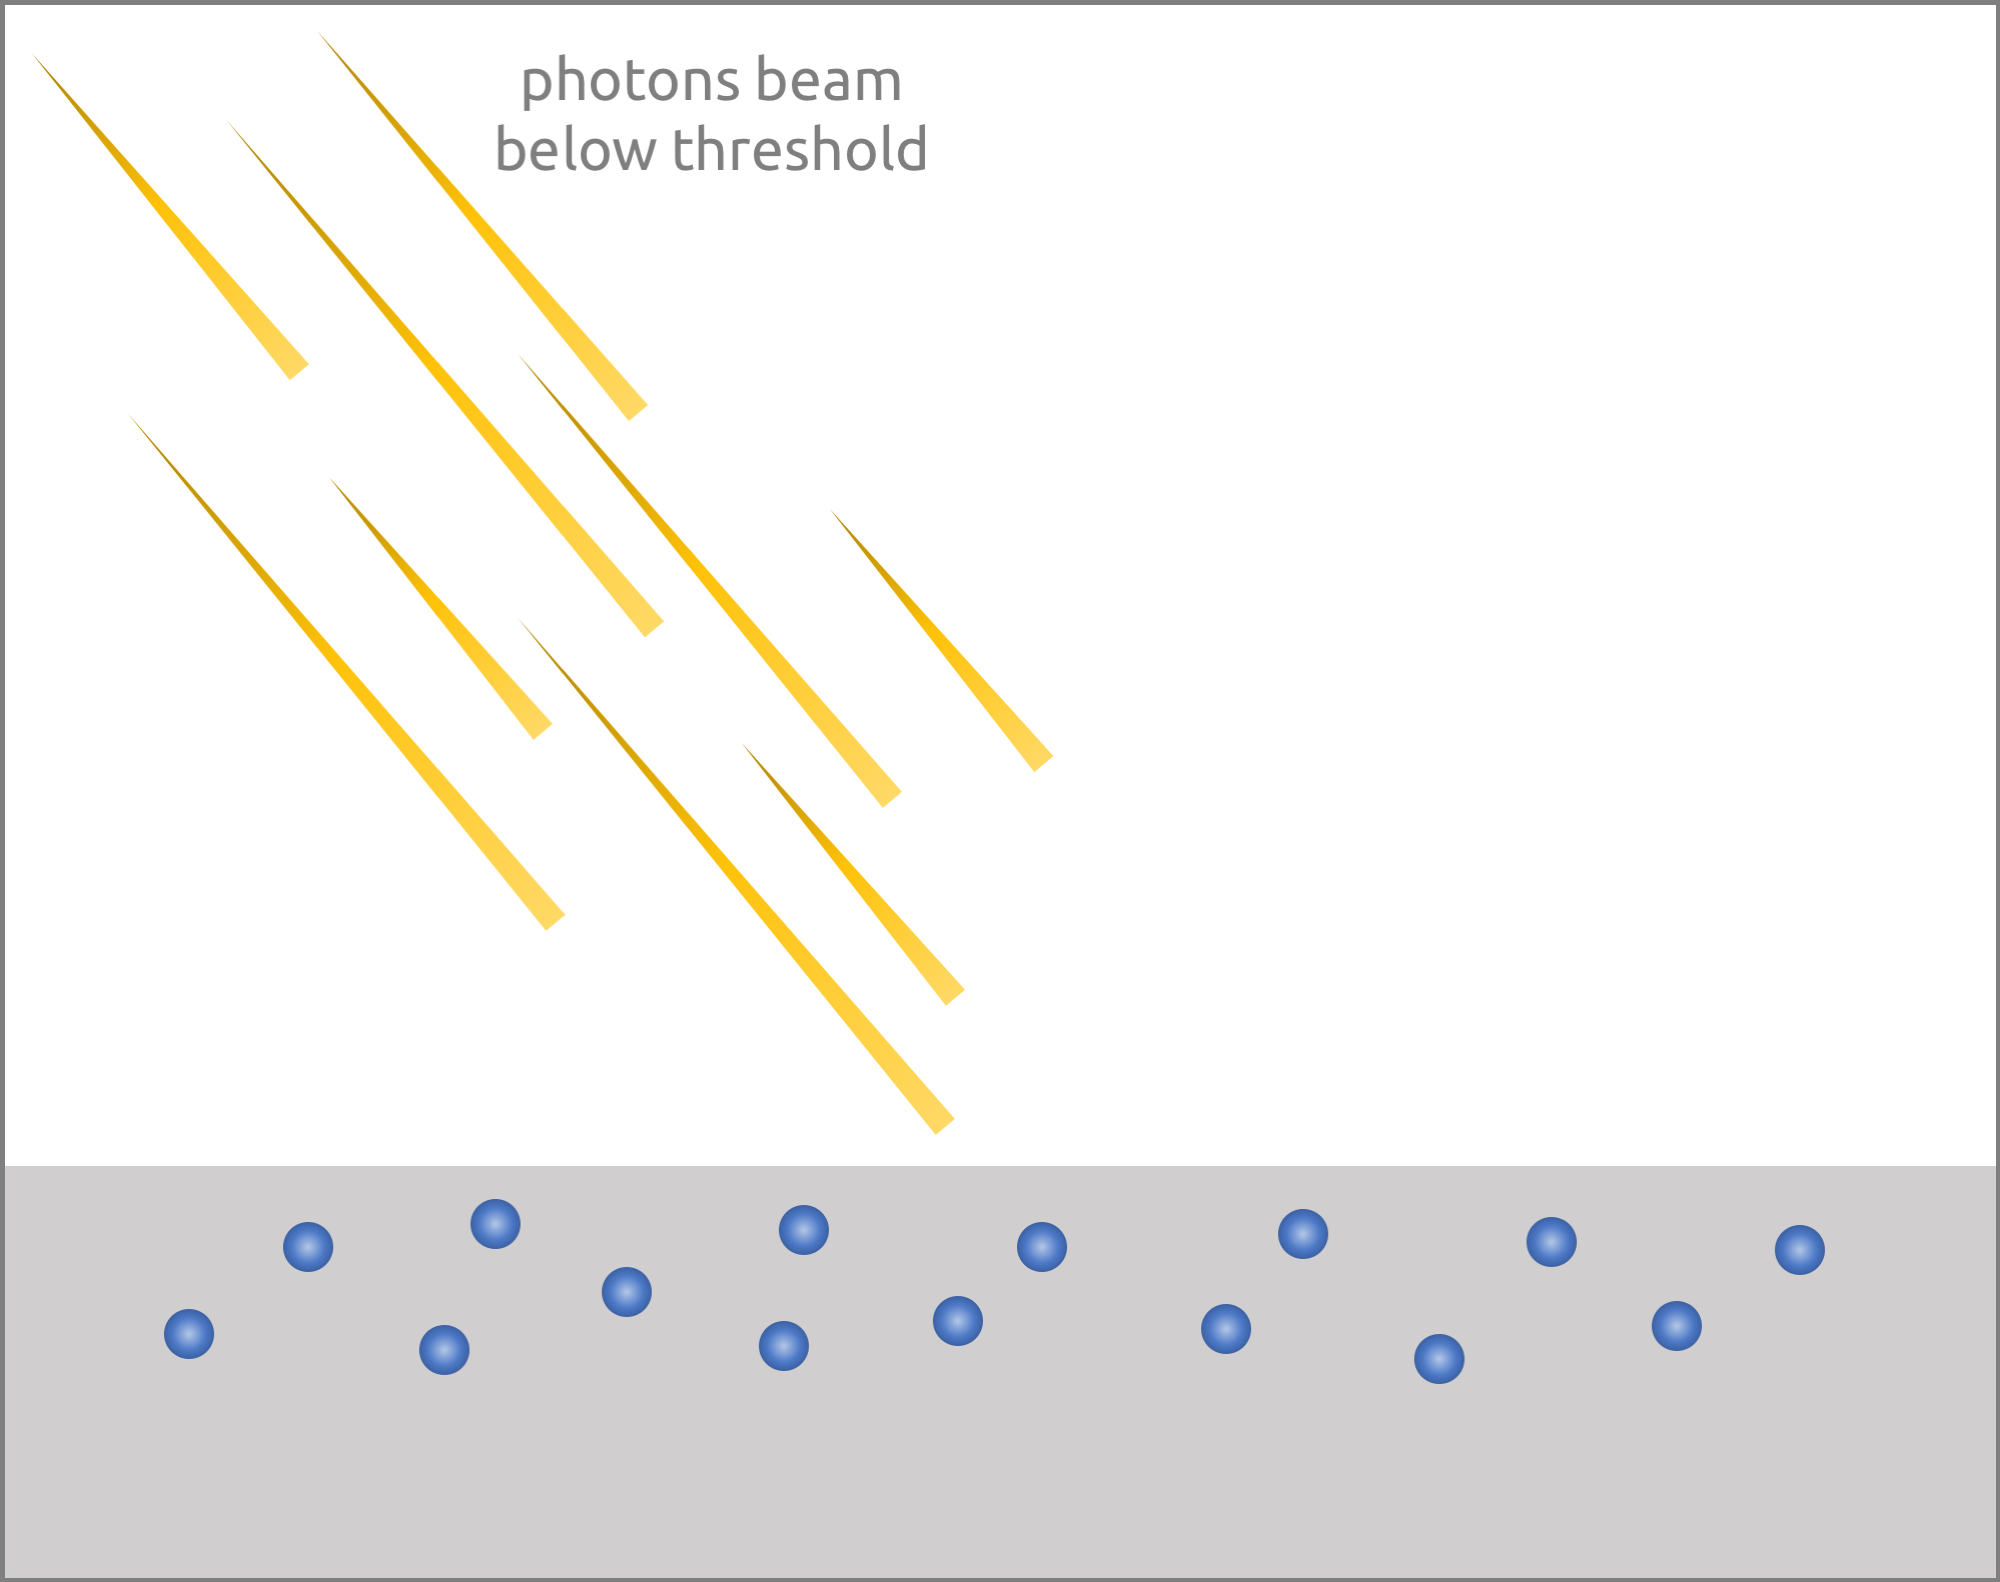
\includegraphics[width=0.48\textwidth]{figures/below2.png}
				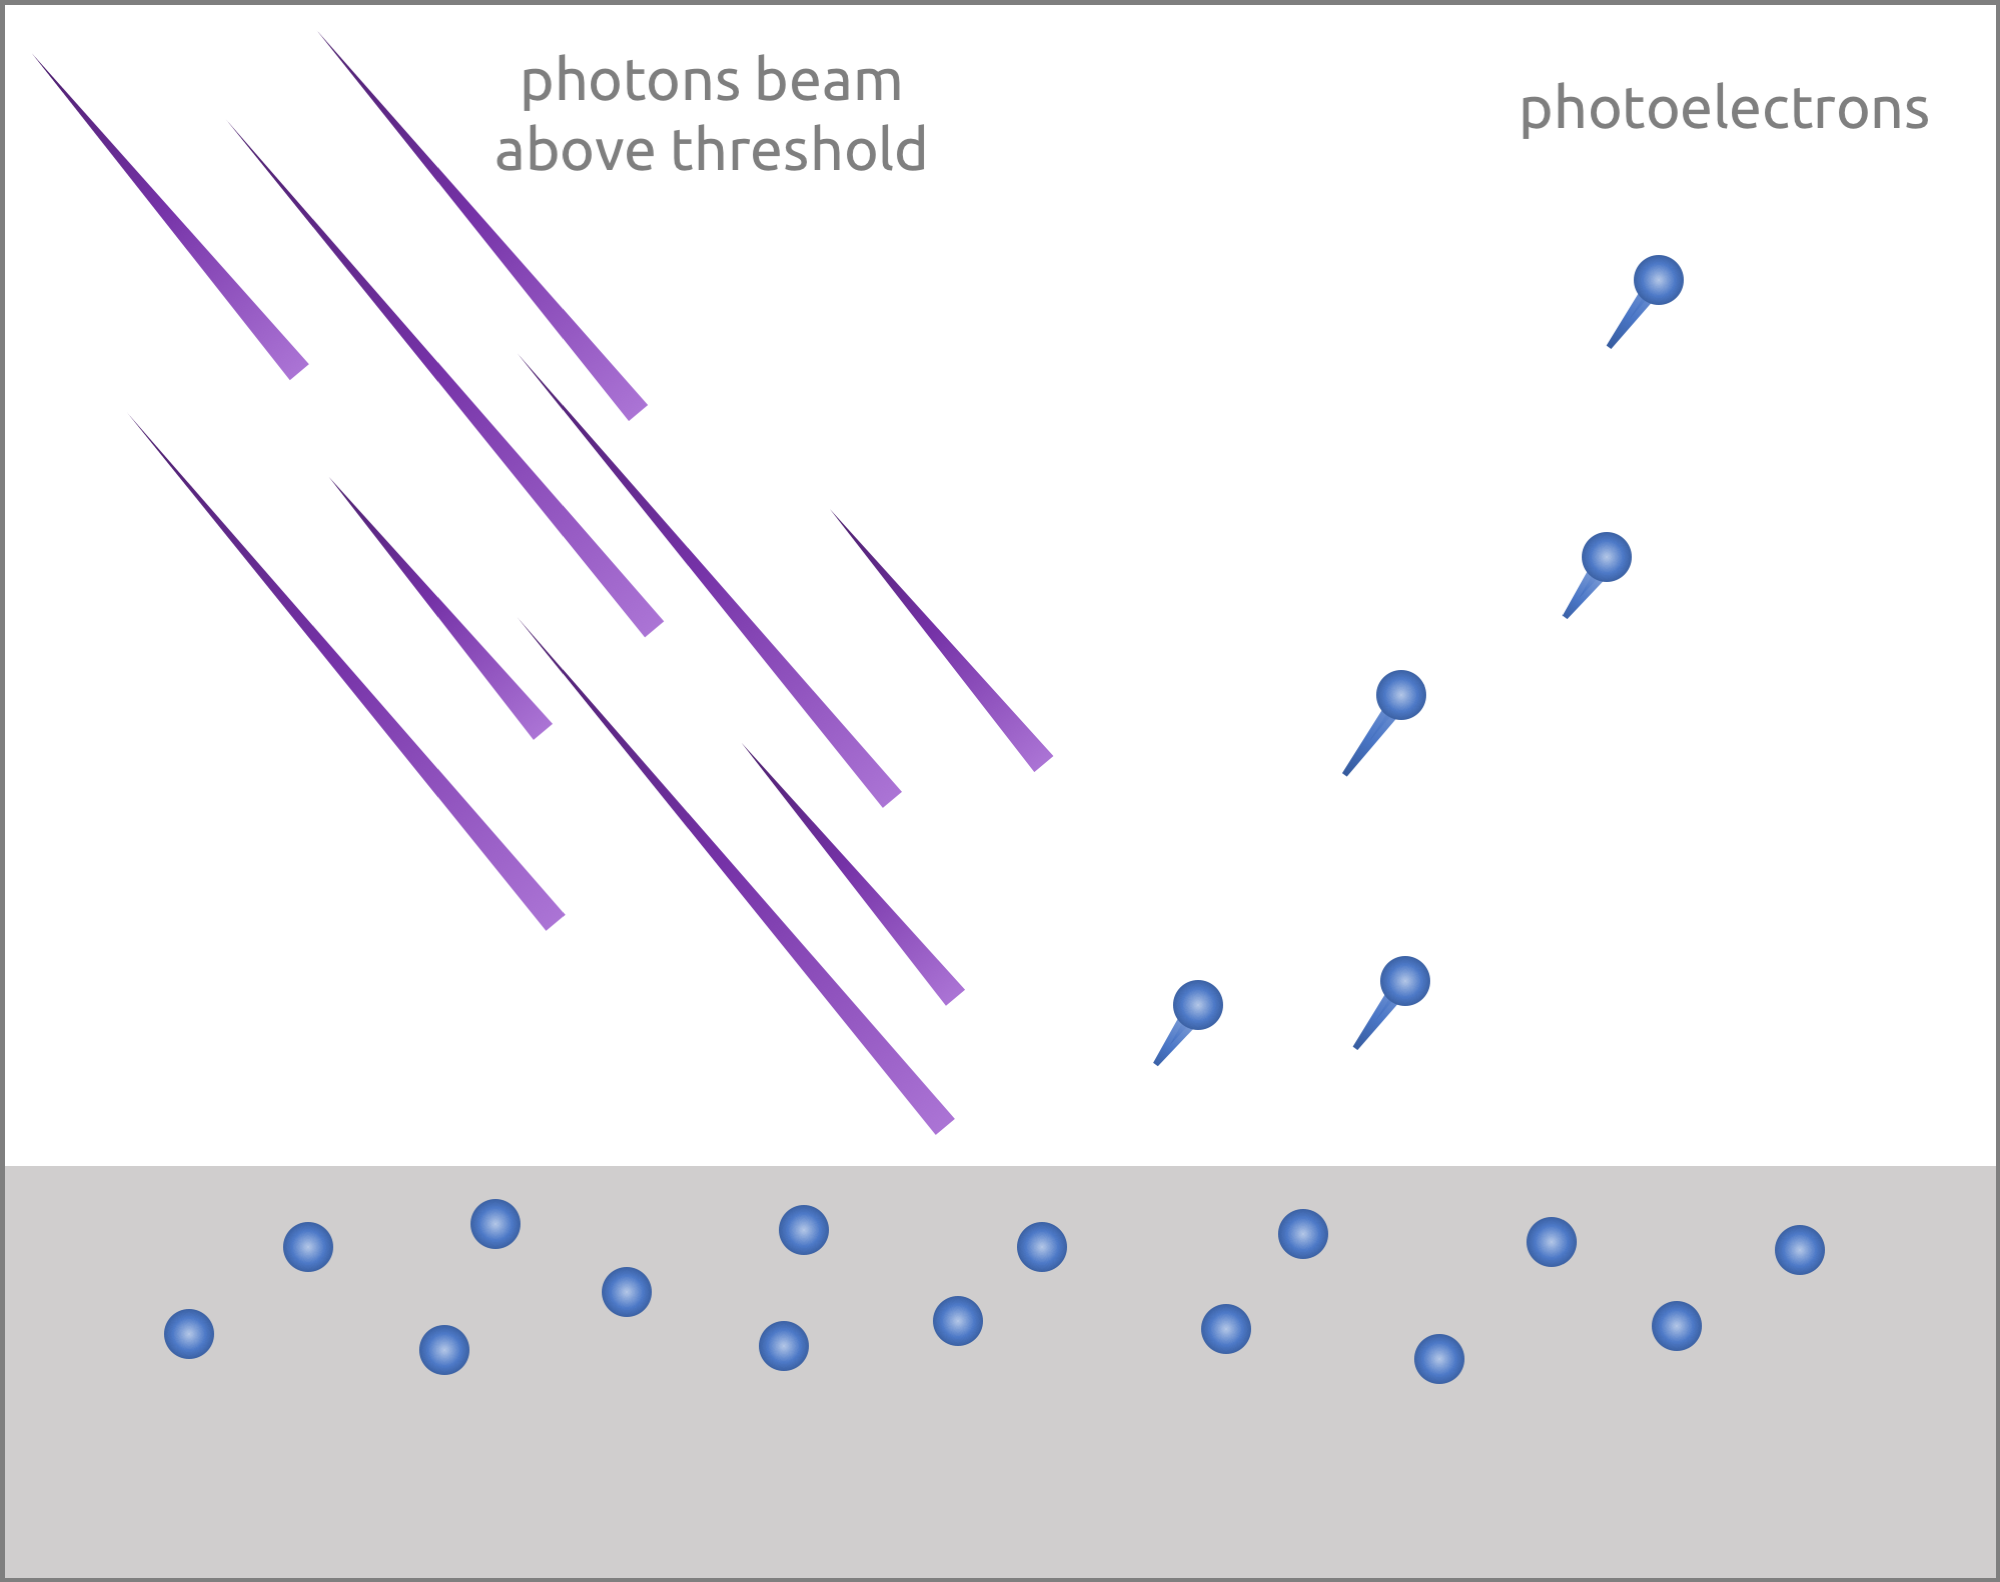
\includegraphics[width=0.48\textwidth]{figures/above2.png}
				\caption{Esquema del efecto fotoeléctrico para luz incidente por debajo del límite necesario. Fuente: \href{https://gsalvatovallverdu.gitlab.io/post/2017-01-09-photoelectric-effect-gif/}{Germain Salvato Vallverdu}.}
				\label{fig:photo-effect} 
\end{figure}

Cuando los fotones incidentes tienen una energía $ h\nu > \phi $, el exceso de energía ($ h\nu - \phi $) lo adquiere el electrón como energía cinética. Debido a que la energía cinética está dada por $ K = mv^2/2 $, donde $ m $ y $ v $ son la masa y velocidad del electrón, respectivamente, es posible calcular la velocidad máxima a la que son expulsados los electrones mediante la relación:
\[ K_{\max} = h\nu - \phi. \]

\subsubsection{Dispositivos de carga acoplada}
Los CCD son sensores construidos a partir de materiales semiconductores como el silicio (Si) y el germanio (Ge). Se trata de dispositivos sensibles a la luz (foto sensibles) en el rango óptico, que se encargan de convertir dicha luz en señales eléctricas. El principio de funcionamiento de los CCD se basa en el efecto fotoeléctrico y el movimiento de electrones en un material semiconductor: un fotón que golpea al detector puede liberar a un electrón y producir así un hueco, que en otras palabras produce una corriente. 

Los CCD comenzaron a utilizarse en telescopios desde la década de 1970 y son actualmente los dispositivos más utilizados en la astronomía óptica (reemplazando a las placas fotográficas, por ejemplo). Una cámara CCD por ejemplo, consiste de una superficie de diodos de silicio foto sensibles, colocados en un arreglo rectangular de píxeles. 

\subsection{Calibración de imágenes CCD}
Como cualquier otro dispositivo tecnológico, los CCD no son perfectos y de hecho cuentan con problemas técnicos que afectan a los datos recolectados con ellos. Para poder realizar un análisis riguroso de los datos tomados con un CCD primero se necesita llevar a cabo un proceso conocido como <<reducción>>, que en realidad es una calibración. En la siguiente sección se intentará describir por qué es necesaria esta calibración

\subsubsection{Funtes de ruido en un CCD}
Toda imagen astronómica está compuesta de un arreglo bidimensional de valores numéricos. Idealmente se esperaría que el valor de cada píxel fuese directamente proporcional a la cantidad de luz recibida en ese píxel mientras la cámara estuvo funcionando. Lamentablemente esto no es así. Para más detalles, puedes revisar el texto <<Handbook of CCD Astronomy>> de \citet{howell2006handbook}.

El valor numérico almacenado en los píxeles de las imágenes astronómicas es llamado \emph{Unidad Digital Análoga} (ADU, por sus siglas en inglés), o simplemente <<\emph{conteo}>>. Los conteos en los que estamos interesados son aquellos que se generaron por efecto fotoeléctrico cuando la luz golpeó al detector. La cantidad de fotones en cada píxel se relaciona con los conteos del píxel mediante un parámetro llamado <<ganacia>>. Sin embargo, intentar convertir los conteos de una imagen a fotones/electrones no tiene sentido, ya que existen muchas contribuciones en los conteos de cada píxel que no se deben a la luz. Esas contribuciones son:

\begin{itemize}
  \item El \textbf{bias}, es un nivel de señal eléctrica que se añade intencionadamente a cada píxel durante el proceso de lectura. Este offset garantiza que las cuentas (valores numéricos de los píxeles) sean siempre positivas, incluso en ausencia de señal luminosa (por ejemplo, cuando el CCD no ha recibido fotones). Este voltaje de bias evita que los errores de lectura o fluctuaciones electrónicas generen valores negativos, lo que no tiene sentido en el contexto de un sensor que cuenta fotones.

  \item El \textbf{dark current} o corriente oscura es una señal generada en los píxeles de un CCD debido al movimiento térmico de los electrones, incluso en ausencia de luz (fotones). Este fenómeno ocurre porque los electrones pueden ser excitados térmicamente dentro del material semiconductor del CCD, creando una señal que es indistinguible de una señal generada por la luz.
  
  \item El \textbf{read noise} es un tipo de ruido inherente a la electrónica del CCD y se genera durante el proceso de \textbf{lectura de los píxeles}. Este ruido se produce principalmente cuando las cargas acumuladas en los píxeles se convierten en una señal digital que puede ser procesada por una computadora. Aunque es imposible eliminar completamente el read noise, se puede minimizar optimizando la electrónica del CCD y enfriando el detector
  
  \item El \textbf{sky background} es la luz que se observa desde el cielo nocturno y que no proviene de los objetos astronómicos que se están estudiando. Este fenómeno ocurre debido a la \textbf{dispersión de la luz} en la atmósfera terrestre y otras fuentes ambientales, y puede afectar la calidad de las observaciones.
  
  \item Los \textbf{rayos cósmicos} son partículas de alta energía provenientes del espacio, que pueden interactuar con los detectores CCD durante las observaciones astronómicas. Cuando estas partículas inciden en el CCD, liberan una carga eléctrica en los píxeles que, al ser leída por el sistema, se convierte en cuentas (counts) que parecen señal, aunque en realidad no lo son.
  
  \item Los CCDs también presentan variaciones en la sensibilidad de cada píxel y como resultado, las imágenes se ven afectadas, haciendo que algunas regiones se vean más oscuras o más brillantes que otras. La fuente más común que genera estas variaciones es el polvo en las lentes o filtros. 
\end{itemize}

La reducción de datos astronómicos consiste esencialmente en eliminar todas estas fuentes de ruido en los píxeles para quedarse únicamente con la luz que proviene de los objetos astronómicos. 

\subsubsection{Proceso de reducción}
La fuente ruido más simple de corregir es el bias, ya que se trata de un valor constante en todos los píxeles de la CCD. Para conocer el valor constante en la imagen CCD, se debe tomar una imagen con un tiempo de exposición cero y con el obturador cerrado. Esto es porque el propósito es únicamente capturar el offset electrónico inherente al CCD, sin ninguna contribución de luz. 

Otra fuente de ruido que es sencilla de corregir es el sky background. Lo único que se debe hacer es estimar el valor del fondo del cielo en áreas libres de objetos astronómicos. Por otro lado, una forma de reducir los efectos de la corriente oscura es enfriando el CCD. Al reducir la temperatura del detector, el movimiento térmico de los electrones disminuye significativamente. Sin embargo, nunca se elimina por completo, ya que siempre existe una pequeña cantidad de excitación térmica. En el mejor de los casos y en algunos de los telescopios modernos, este efecto se vuelve despreciable. Si en cambio no es posible reducir los efectos del dark current con la temperatura, se deben tomar imágenes oscuras (o dark frames). Los dark frames se toman con el obturador cerrado, pero a diferencia del bias, se utiliza un tiempo de exposición distinto de cero. Se debe usar el mismo tiempo de exposición con el que se tomaron las imágenes de interés, llamadas también imágenes científicas.

El ruido de lectura es imposible de eliminar, ya que es completamente aleatorio. Además, este ruido está presente en todas las imágenes, incluyendo las de bias y las de corriente oscura. Es posible reducir el ruido de lectura reduciendo la temperatura y mejorando la eficiencia de los CCDs pero estará siempre presente.

Para corregir las no uniformidades o variaciones en la sensibilidad de los detectores se utilizan imágenes de campo plano o \emph{flat fields}. Un flat field se captura apuntando el telescopio hacia una fuente de luz uniforme, que idealmente debería iluminar el detector de manera homogénea en toda la superficie. Las formas más comunes de obtener los flat fields son:
\begin{itemize}
  \item Utilizando paredes iluminadas artificialmente en el observatorio.
  \item Capturando imágenes del cielo del crepúsculo, poco después del atardecer o antes del amanecer.
\end{itemize}

El proceso de corrección por rayos cósmicos consiste en utilizar algoritmos luego de procesar las imágenes. Los algoritmos se encargan de identificar y eliminar el ruido causado por rayos cósmicos. Otra forma de hacerlo es tomar múltiples exposiciones de la misma región del cielo para luego combinarlas y eliminar cualquier rastro de rayos cósmicos que aparezcan en una sola exposición. 
 
Adicionalmente, los CCDs cuentan con una región extra que no está expuesta a la luz, pero que registra valores electrónicos. Dicha región recibe el nombre de \emph{overscan} y puede usarse para monitorear y corregir variaciones en el bias durante la lectura. 

Todas las fuentes de ruido mencionadas anteriormente son aditivas, es decir, que una imagen astronómica sin calibrar está compuesta por múltiples componentes que se suman, de la siguiente manera:
\[ \mathrm{image = bias + noise + dark current + sky + stars} \]

Sin embargo, los efectos de las variaciones en sensibilidad consisten en reducir la cantidad de luz que llega al detector. Esto significa que afecta tanto a la luz que llega de las estrellas y del fondo del cielo. Es decir, que la expresión anterior cambia de la siguiente manera:
\[ \mathrm{image = bias + noise + dark current + flat\times(sky + stars)}, \]
debido a esto, decimos que los flat fields son multiplicativos. 

Ya que estamos interesados únicamente en los conteos provenientes de las estrellas, debemos resolver la ecuación anterior para la variable $ \mathrm{stars} $, entonces:
\[ \mathrm{stars + noise_f = \frac{image - bias - dark current}{flat}  - sky }. \]

Recuerda que el ruido de lectura es imposible de eliminar. En realidad, los dark frames y los flat fields también cuentan con bias. Así que para usar la ecuación anterior, primero se deben corregir ambas cantidades de la siguiente manera:
\[ \mathrm{dark current = \frac{dark frame - bias}{exposure ~ time}}, \]
\[ \mathrm{flat = flat field - bias} \]
 
 
 
